\documentclass[a4paper, 12pt]{article}
\usepackage[utf8]{inputenc}
\usepackage[T1]{fontenc}
\usepackage[french]{babel}
\usepackage{graphicx}
\usepackage{amsmath}
\usepackage{hyperref}
\usepackage{lmodern}
\usepackage{moreverb}
\usepackage{multicol}

\hypersetup{
    colorlinks=true,
    linkcolor=blue,
    filecolor=magenta,      
    urlcolor=cyan,
    pdftitle={Overleaf Example},
    pdfpagemode=FullScreen,
    }

\urlstyle{same}
\usepackage[a4paper,left=2cm,right=2cm,top=2cm,bottom=2cm]{geometry}

\pagestyle{headings}
\pagestyle{plain}


\setcounter{secnumdepth}{4}
\setcounter{tocdepth}{4}
\makeatletter


\makeatother



\makeatletter
\def\toclevel@subsubsubsection{4}
\def\toclevel@paragraph{5}
\def\toclevel@subparagraph{6}
\makeatother





\setlength{\parindent}{0cm}
\setlength{\parskip}{1ex plus 0.5ex minus 0.2ex}
\newcommand{\hsp}{\hspace{20pt}}
\newcommand{\HRule}{\rule{\linewidth}{0.5mm}}

\begin{document}

\begin{titlepage}
  \begin{sffamily}
  \begin{center}

   
    \textsc{\LARGE }\\[2cm]

    \textsc{\Large Compte rendu de Réunion}\\[1.5cm]
    \textsc{\Medium Rédigé par Ghilas Meziane}

    % Title
    \HRule \\[0.4cm]
    { \huge  \textsc{StellaStone} \\
    \textsc{\Large By Novus}\\ [0.4cm] }
	

    \HRule \\[2cm]
    \textsc {Idriss BENGUEZZOU\\Mohammed ROUABAH\\Ghilas MEZIANE \\ Ilyes ZEGHDALLOU}
 \begin{figure}
     \centering
    
\includegraphics[scale=0.2]{logoUJM.png}
     \label{fig:ujm_logo}
 \end{figure}
   
    \

    \vfill

    % Bottom of the page
    {\large {} 17/10/2022}

  \end{center}
  \end{sffamily}
\end{titlepage}

\newpage

\section{Réunion du Vendredi 14/10}
Nous nous sommes réunis le vendredi 14 octobre 2022. Cette réunion a pu être tenue cette fois ci en présentiel, dans une salle de cours libre sur le campus Manufacture, avec la présence de tous les membres, sur le créneau horaire 17h-18h, juste après le TP d'algorithmique avancée.

\section{Fusion des documents}

Nous avons dans un premier temps discuté des exigences que chacun a pu rédiger durant la semaine. L'ordre du jour était de faire une relecture du document de spécifications des exigences. Nous avons pu remarquer que certaines idées étaient contradictoires et incohérentes. C'est pourquoi nous avons décidé de revoir ensemble la structure générale du projet pour repartir sur de bonnes bases, ce qui a donné lieu à la suppression de certaines exigences et à la création d'autres.

\section{Une première visualisation}
Il est plus facile de rédiger des exigences lorsque l'on a une vision générale claire du projet. C'est pourquoi nous avons eu l'idée de dessiner, sur le tableau de la salle de cours dans laquelle nous étions présents, une esquisse représentant l'ossature de notre application. En d'autres mots nous avons essayé de représenter les potentielles interfaces de notre logiciel ainsi que les relations entre celles-ci. 

 \begin{figure}[!h]
    \centering
    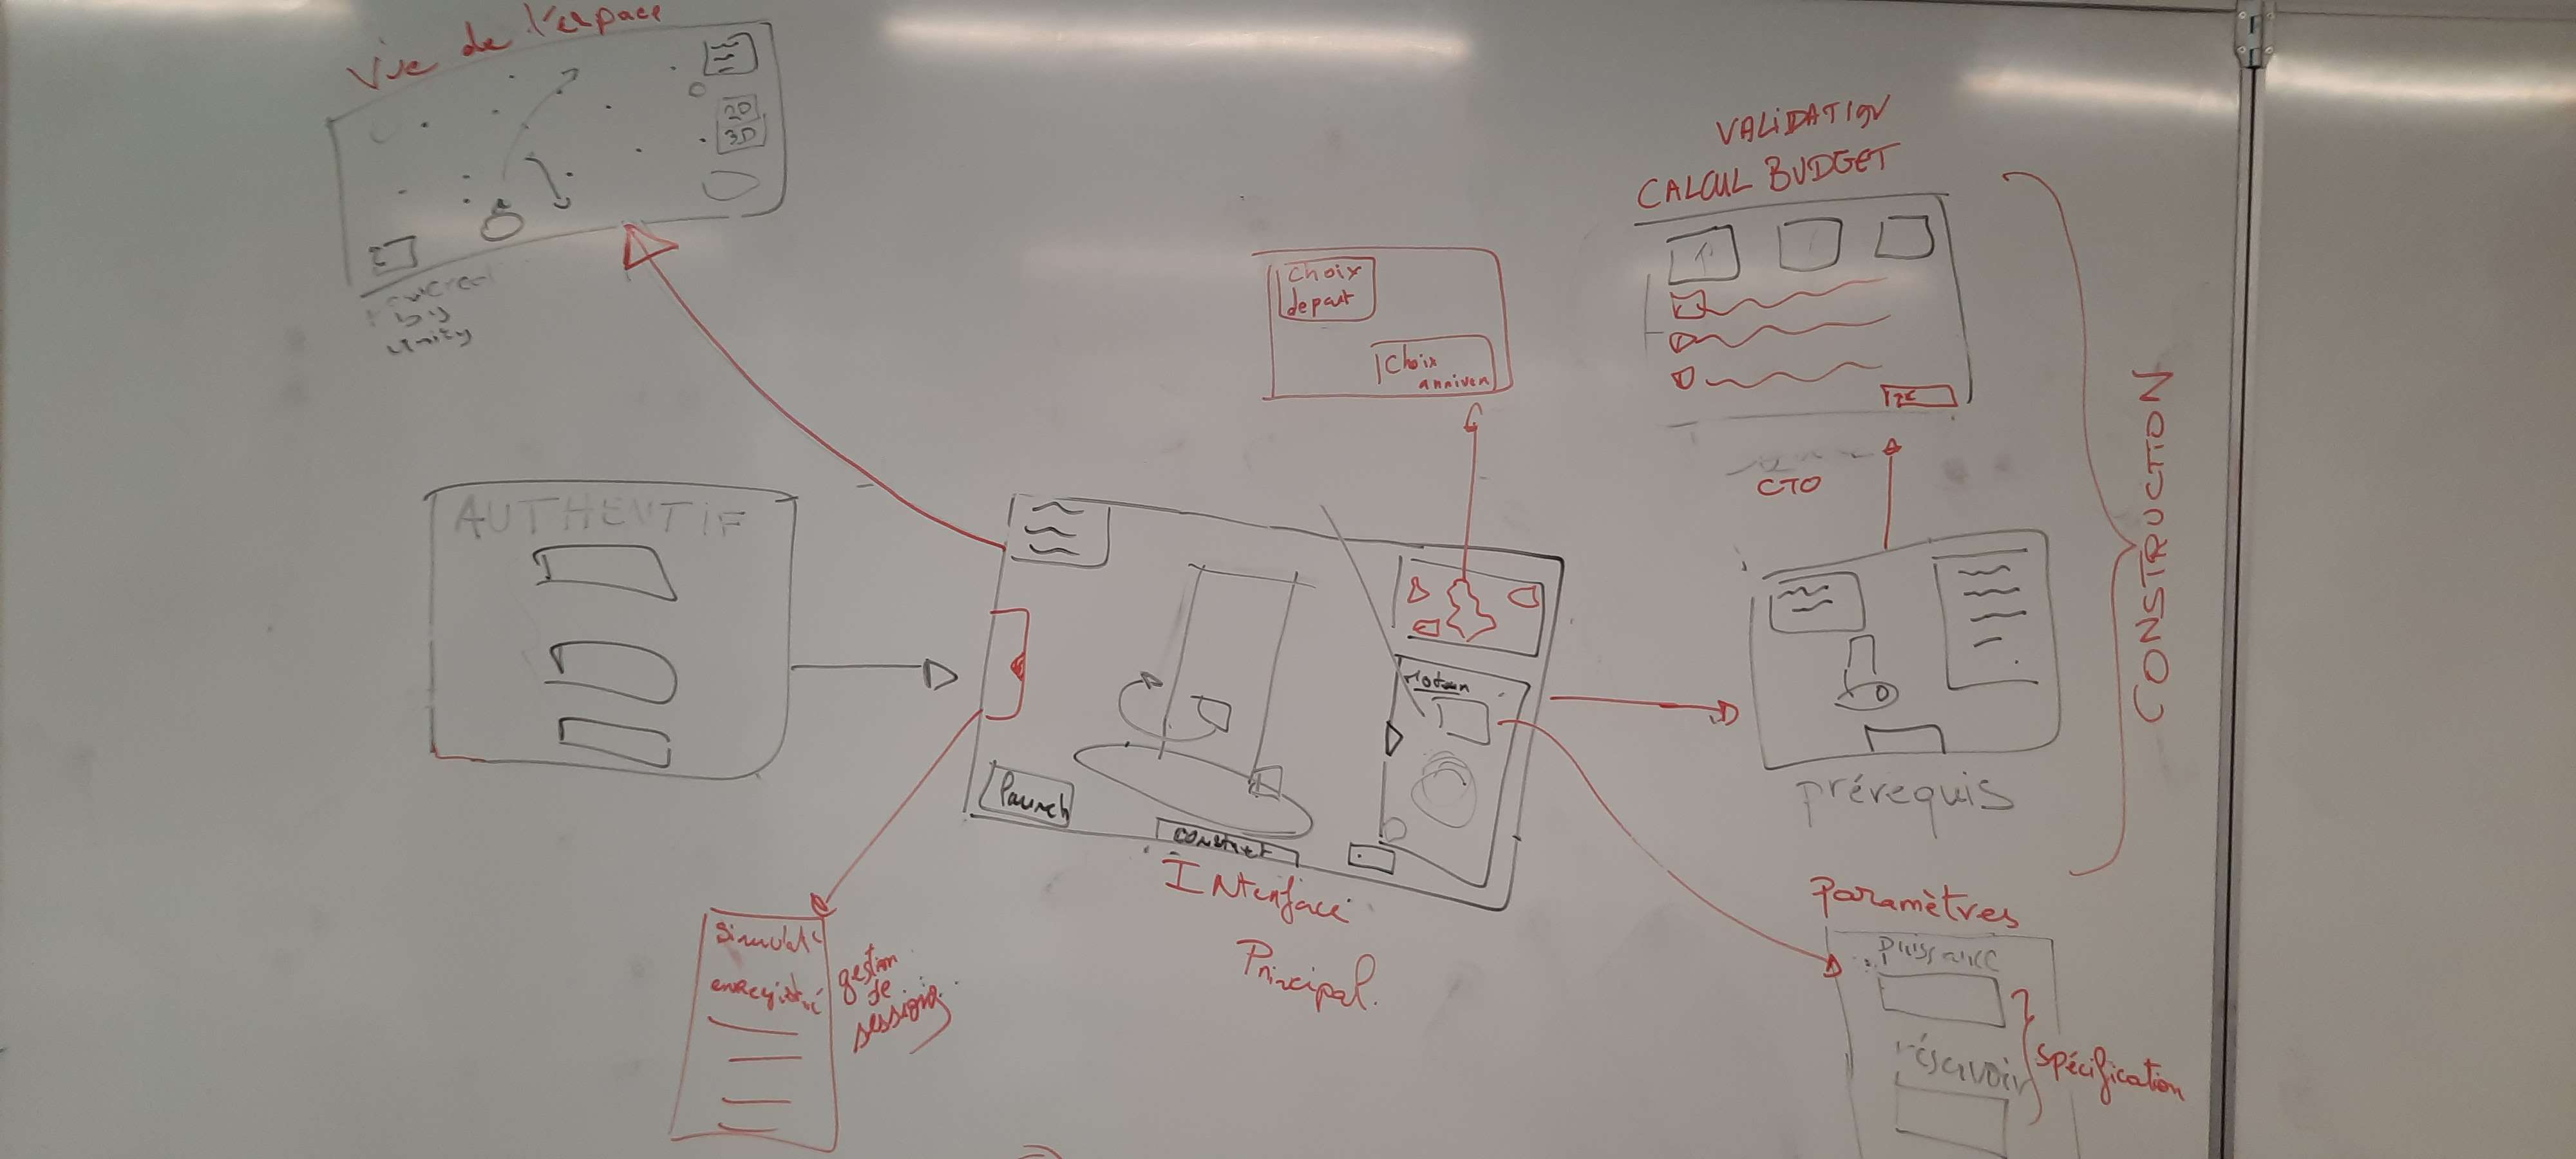
\includegraphics[scale=0.1]{schema.jpg}
    \label{fig:Le_planning}
    \caption{Un premier Schéma du logiciel}
\end{figure} 
\\ \\

L'idée principale proposée par Mr.ROUABAH était de créer tout un tas de rôles, tels que ADMINISTRATEUR, TECHNICIENS, INGÉNIEURS, avec des interfaces assignées à chacun. Le logiciel deviendrait alors une sorte de simulation collaborative, avec une hiérarchie telle une vraie entreprise spatiale, ou par exemple un comptable devrait chiffrer les coûts avant qu'un testeur ne vienne valider....

Mr.BENGUEZZOU a exposé ses inquiétudes quant à cette idée, car elle nous éloignait de l'idée du simulateur. Il a proposé une alternative à cela : par exemple l'idée du comptable qui devrait rédiger un rapport pourrait être remplacée par une interface 'comptabilité' qui générerait ce rapport automatiquement en fonction des composant et choix réalisé par l'utilisateur. 
\\ Ainsi, l'idée de simulation s'étendrait également aux fonctionnalités proposées par Mr.ROUABAH. Cette proposition a été validé par tout le groupe.

Mr.MEZIANE a quant à lui émis des doutes concernant la disponibilité des ressources et l'accessibilité à l'info concernant ce domaine notamment pour le cas des pièces (leur puissances , leurs prix ...) qui sont en général des éléments dont les propriétés ne sont pas partagées au grand public. Mr.ZEGHDALLOU a évoqué qu'il existait certaines normes et contraintes pour les entreprises qui se devaient de rendre publiques certaines informations. De plus, le projet ayant un but ludique, l'inexactitude de certaines données ne serait pas très contraignant.


\section{Prochaine réunion}
La prochaine réunion est fixée pour le vendredi 21 octobre 2021, sur le créneau horaire 17h-18h avec pour ordre du jour: Visualisation de l'avancement du document de spécifications des exigences. Avec pour objectif de la semaine de continuer le document de spécification des exigences tout en commençant en parallèle la rédaction du documents Tests de recette. PTDR TU FOUS QUOI ICI IDRISS
\section{Mise à jour du diagramme de Gantt} 

En dernier lieu, nous avons de nouveau mis à jour le diagramme de Gantt.
Certaines dates ont été revues et des phases ont été ajoutées notamment la phase de relecture de nos documents ainsi que la phase de préparation à la soutenance.
\\\\
 \begin{figure}[!h]
    \centering
    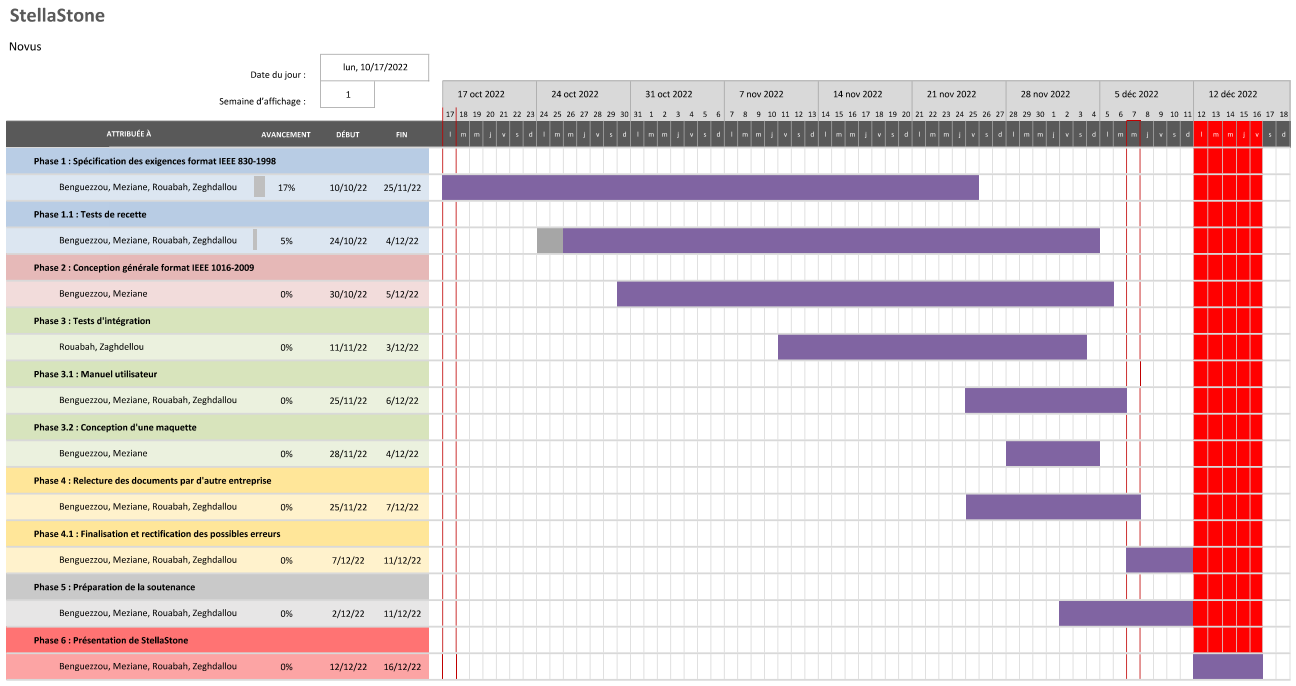
\includegraphics[scale=0.5]{Diagramme de gantt.png}
    \label{fig:Tache_semaine}
    \caption{Diagramme de Gantt}
\end{figure}

\end{document}